%!TEX root = ./main.tex
El primer caso de un grupo de trenzas no abeliano es $B_3$ que definido a partir de relaciones y generadores posee la siguiente presentacion
$$B_3=\langle\sigma_1,\sigma_2\,|\,\sigma_1\sigma_2\sigma_1=\sigma_2\sigma_1\sigma_2\rangle.$$
Geometricamente recordemos que esta relacion se traduce en el movimiento $\Omega_3$, Por el Ejemplo 2.12 (particularmente) y el Teorema 2.20 (general) sabemos que $B_3$ es no abeliano que ya en si es un hecho relevante, pero en esta seccion iremos un poco mas alla respecto a este grupo.\\

Definamos
    $$x=\sigma_1\sigma_2\sigma_1\hspace{5mm}y=\sigma_1\sigma_2$$
    Note que $x=y\sigma_1$, luego $\sigma_1=y^{-1}x,$ mientras que $$\sigma_2=\sigma_1^{-1}x\sigma_1^{-1}=(x^{-1}y)x(x^{-1}y)=x^{-1}y^2$$
    Luego como ambos generadores los podemos reescribir en términos de $x$ y $y$ tenemos la siguiente presentación equivalente
    $$B_3=\langle x,y\,|\,x^2=y^3\rangle$$
    con esto podemos probar particularmente para este caso que
    \begin{prop}
        El centro de $B_3$ es generado por $y^3$, es decir
        $$Z(B_3)=\langle y^3\rangle$$
    \end{prop}
    \begin{proof}
        Para mostrar que un elemento esta en el centro basta ver que conmuta con los generadores, es claro que $y^3$ conmuta con $y$, ahora note que $xy^3=xx^2=x^3=x^2x=y^3x,$ así $y^3\in Z(B_3)$ y por tanto $\langle y^3\rangle\subset Z(B_3).$\\
    Como el centro de cualquier grupo es normal, $\langle y^3\rangle$ también lo es, luego
    $$B_3/\langle y^3\rangle=\langle x,y|x^2=y^3=1\rangle=\Z_2*\Z_3$$ Asi el centro es trivial, es decir $Z(B_3/\langle y^3\rangle)=\{\langle y^3\rangle\}$. Con esto sea $b\in Z(B_3)$, eso implica que $bg=gb$ para todo $g\in B_3$, así $bg\langle y^3\rangle=gb\langle y^3\rangle$, lo que implica que la clase lateral $b\langle y^3\rangle\in Z(B_3/\langle y^3\rangle)$, pero por lo anterior $b\langle y^3\rangle=\langle y^3\rangle$, asi $b\in \langle y^3\rangle$ y concluimos la igualdad.
    \end{proof}

    Con esto en mente consideremos $SL(2,\Z)$, que es el grupo de matrices invertibles con entradas enteras y determinante 1. Un hecho que no probaremos es que $SL(2,\Z)=\left\langle\begin{pmatrix}
        1 & 1\\
        0 & 1
    \end{pmatrix},\begin{pmatrix}
        1 & 0\\
        -1& 1
    \end{pmatrix}\right\rangle$
    La escogencia de estas dos matrices es por lo siguiente:
    \begin{prop}
        Dado $SL(2,\Z)=\left\langle\begin{pmatrix}
        1 & 1\\
        0 & 1
    \end{pmatrix},\begin{pmatrix}
        1 & 0\\
        -1& 1
    \end{pmatrix}\right\rangle$, tenemos que $$Z(SL(2,\Z))=\langle-I_2\rangle$$ y que los dos generadores dados satisfacen las relaciones de trenzas.
    \end{prop}
    \begin{proof}
        La segunda parte es una verificacion sencilla de los productos
        $$\begin{pmatrix}
        1 & 1\\
        0 &1 
    \end{pmatrix}\begin{pmatrix}
        1 & 0\\
        -1 &1 
    \end{pmatrix}
    \begin{pmatrix}
        1 & 1\\
        0 &1 
    \end{pmatrix}=\begin{pmatrix}
        0 & 1\\
        -1 &0 
    \end{pmatrix}=\begin{pmatrix}
        1 & 0\\
        -1 &1 
    \end{pmatrix}
    \begin{pmatrix}
        1 & 1\\
        0 &1 
    \end{pmatrix}\begin{pmatrix}
        1 & 0\\
        -1 &1 
    \end{pmatrix}$$
    Para la primera parte si tomamos una matriz en el centro en particular conmuta con nuestros generadores, es decir
    $$\begin{pmatrix}
        1 & 1\\
        0 & 1
    \end{pmatrix}\begin{pmatrix}
        a & b\\
        c & d
    \end{pmatrix}=\begin{pmatrix}
        a+c & b+d\\
        c & d
    \end{pmatrix}=\begin{pmatrix}
        a & a+b\\
        c & c+d
    \end{pmatrix}=\begin{pmatrix}
        a & b\\
        c & d
    \end{pmatrix}\begin{pmatrix}
        1 & 1\\
        0 & 1
    \end{pmatrix}$$
    De aqui concluimos que $a+c=c$, asi $c=0$, de manera similar $b+d=a+b$, asi $a=d$, asi nuestra matriz sew reduce a $\begin{pmatrix}
        a & b\\
        0 & a\\
    \end{pmatrix}$
    Por la condicion del determinante sabemos que $a=\pm 1$ falta ver que ocurre con $d$, pero
    $$\begin{pmatrix}
        1 & 0\\
        -1 & 1
    \end{pmatrix}\begin{pmatrix}
        a & b\\
        0 & a
    \end{pmatrix}=\begin{pmatrix}
        a & b\\
        -a & -b+a
    \end{pmatrix}=\begin{pmatrix}
        a-b & b\\
        -a & a
    \end{pmatrix}=\begin{pmatrix}
        a & b\\
        0 & a
    \end{pmatrix}\begin{pmatrix}
        1 & 0\\
        -1 & 1
    \end{pmatrix}$$
    Esto implica que $a-b=a$ y por tanto $b=0$, asi concluimos lo deseado.

    \end{proof}
    Observe entonces que el grupo modular $PSL(2,\Z):=SL(2,\Z)/Z(SL(2,\Z))$, tendra centro trivial ya que las clases solo difieren por signo. Con esto en mente tenemos el resultado deseado de $B_3$
    \begin{theorem}
        Dados $B_3$ y $SL(2,\Z)$ existe un unico homomorfismo, que desciende en un isomorfismo
        $$B_3/Z(B_3)\cong PSL(2,\Z).$$
    \end{theorem}
    \begin{proof}
        La existencia esta garantizada por \ref{homoexis}, asi tenemos que $\sigma_1\mapsto A=\begin{pmatrix}
        1 & 1\\
        0 & 1
    \end{pmatrix}$ y $\sigma_2\mapsto B=\begin{pmatrix}
        1 & 0\\
        -1 & 1
    \end{pmatrix}$, observe que este es sobreyectivo ya que las matrices generan el grupo especial lineal, luego la composicion con la proyeccion a $PSL(2,\Z)$ tambien es sobreyectiva. Tenemos que $x\mapsto S=\begin{pmatrix}
        0 & 1\\
        -1 &0 
    \end{pmatrix}$, luego $x^2\mapsto -I_2$, asi $x^2$ esta contenido en el kernel del homomorfismo, y por tanto se induce un homomorfismo como en el siguiente diagrama.
    \begin{center}
        

\tikzset{every picture/.style={line width=0.75pt}} %set default line width to 0.75pt        

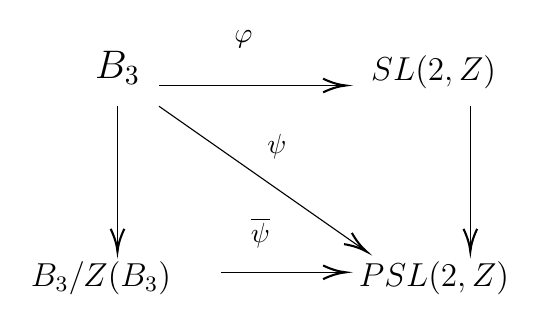
\begin{tikzpicture}[x=0.75pt,y=0.75pt,yscale=-1,xscale=1]
%uncomment if require: \path (0,877); %set diagram left start at 0, and has height of 877

%Straight Lines [id:da11668079361738581] 
\draw    (210,120) -- (298,120) ;
\draw [shift={(300,120)}, rotate = 180] [color={rgb, 255:red, 0; green, 0; blue, 0 }  ][line width=0.75]    (10.93,-3.29) .. controls (6.95,-1.4) and (3.31,-0.3) .. (0,0) .. controls (3.31,0.3) and (6.95,1.4) .. (10.93,3.29)   ;
%Straight Lines [id:da060790583995789405] 
\draw    (360,130) -- (360,198) ;
\draw [shift={(360,200)}, rotate = 270] [color={rgb, 255:red, 0; green, 0; blue, 0 }  ][line width=0.75]    (10.93,-3.29) .. controls (6.95,-1.4) and (3.31,-0.3) .. (0,0) .. controls (3.31,0.3) and (6.95,1.4) .. (10.93,3.29)   ;
%Straight Lines [id:da8757010499358835] 
\draw    (210,130) -- (308.36,198.85) ;
\draw [shift={(310,200)}, rotate = 214.99] [color={rgb, 255:red, 0; green, 0; blue, 0 }  ][line width=0.75]    (10.93,-3.29) .. controls (6.95,-1.4) and (3.31,-0.3) .. (0,0) .. controls (3.31,0.3) and (6.95,1.4) .. (10.93,3.29)   ;
%Straight Lines [id:da8152415293734984] 
\draw    (240,210) -- (298,210) ;
\draw [shift={(300,210)}, rotate = 180] [color={rgb, 255:red, 0; green, 0; blue, 0 }  ][line width=0.75]    (10.93,-3.29) .. controls (6.95,-1.4) and (3.31,-0.3) .. (0,0) .. controls (3.31,0.3) and (6.95,1.4) .. (10.93,3.29)   ;
%Straight Lines [id:da5884397458751206] 
\draw    (190,130) -- (190,198) ;
\draw [shift={(190,200)}, rotate = 270] [color={rgb, 255:red, 0; green, 0; blue, 0 }  ][line width=0.75]    (10.93,-3.29) .. controls (6.95,-1.4) and (3.31,-0.3) .. (0,0) .. controls (3.31,0.3) and (6.95,1.4) .. (10.93,3.29)   ;

% Text Node
\draw (178,102.4) node [anchor=north west][inner sep=0.75pt]  [font=\Large]  {$B_{3}$};
% Text Node
\draw (311,104.4) node [anchor=north west][inner sep=0.75pt]  [font=\large]  {$SL( 2,\mathbb{Z})$};
% Text Node
\draw (305,203.4) node [anchor=north west][inner sep=0.75pt]  [font=\large]  {$PSL( 2,\mathbb{Z})$};
% Text Node
\draw (245,92.4) node [anchor=north west][inner sep=0.75pt]    {$\varphi $};
% Text Node
\draw (261,142.4) node [anchor=north west][inner sep=0.75pt]    {$\psi $};
% Text Node
\draw (253,182.4) node [anchor=north west][inner sep=0.75pt]    {$\overline{\psi }$};
% Text Node
\draw (147,203.4) node [anchor=north west][inner sep=0.75pt]  [font=\large]  {$B_{3} /Z( B_{3})$};


\end{tikzpicture}

    \end{center}
    Nos bastaría mostrar que $\overline{\psi}$ es inyectiva. Por la presentación cualquier elemento tendrá la siguiente forma
    $$\omega=y^{\pm1}x\cdots y^{\pm1}xy^{\pm1}, \omega x,x\omega, x\omega x, x$$
    Es claro que $x$ no estaría en el kernel. Luego como $x\omega x=x\omega x^{-1}$, es decir, es conjugado de $\omega$ y $x\omega$ es conjugado de $\omega x$, basta ver que $\omega$y $\omega x$ no están en el kernel.
    Por las presentaciones
    $y^{-1}x\mapsto \overline{A}$ y $yx\to \overline{B}^{-1}$. Así $\overline{\psi}(\omega x)$ es un producto de matrices $A,B^{-1}$, pero note que cualquier producto no vació de estas tiene entradas en la diagonal mayor a $1$, así no podrá ser la identidad, de manera similar si $\overline{\psi}(\omega)=I$ entonces $\overline{\psi}(\omega x)=\overline{\psi}(x)=S$, pero esto es imposible por la condición sobre las entradas, así la función es inyectiva y hemos probado que
    $$B_3/Z(B_3)\cong PSL(2,\Z).$$
    \end{proof}
